%%%%%%%%%%%%%%%%%%%%%%%%%%%%%%%%%%%%%%%%%%%%%%%%%%%%%%%
%                  File: OPTICAmeetings.tex           %
%                  Date: 31 July 2023                 %
%                                                     %
%     For preparing LaTeX manuscripts for submission  %
%     submission to Optica meetings and conferences   %
%                                                     %
%         (c) 2018-2022 Optica Publishing Group       %
%%%%%%%%%%%%%%%%%%%%%%%%%%%%%%%%%%%%%%%%%%%%%%%%%%%%%%%

\documentclass[letterpaper, 12pt]{article} 
%% if A4 paper needed, change letterpaper to A4

%% provide authormark
\newcommand\authormark[1]{\textsuperscript{#1}}

%% standard packages and arguments should be modified as needed
\usepackage{amsmath,amssymb}
\usepackage[colorlinks=true,bookmarks=false,citecolor=blue,urlcolor=blue]{hyperref} %pdflatex
%\usepackage[breaklinks,colorlinks=true,bookmarks=false,citecolor=blue,urlcolor=blue]{hyperref} %latex w/dvipdf
\usepackage{hanging}
\usepackage{changepage}
\usepackage{url}
\usepackage{graphicx}
\usepackage{authblk}
\usepackage{setspace}
\usepackage[english]{babel}
\usepackage[autostyle, english = american]{csquotes}
\MakeOuterQuote{"}
\usepackage{dirtytalk}
\title{\vspace{-2.0cm}Stuff}

\renewenvironment{abstract}
 {\small
  \begin{center}
  \bfseries \abstractname\vspace{-.5em}\vspace{0pt}
  \end{center}
  \list{}{%
    \setlength{\leftmargin}{3mm}% <---------- CHANGE HERE
    \setlength{\rightmargin}{\leftmargin}%
  }%
  \item\relax}
 {\endlist}

\begin{document}
\doublespacing
% \author{Author name(s)}
% \address{Author affiliation and full address}
% \email{e-mail address}
%%Uncomment the following line to override copyright year from the default current year.
%\copyrightyear{2024}

\title{\vspace{-1cm} Speech Enhancement and De-noising for Classification Tasks.}
\author{Preethi Natesan Sridhar, Samuel Merten, Shrivats Sudhir, Srivats Kumar Taralinath.}
\date{December 13, 2023.}

\maketitle

\begin{abstract}
This report is intended to explore the use of unsupervised isolation- and density-based ensemble models for anomaly detection and cleaning using speech data. Furthermore, the paper also shows neural network classification implemented to quantify model performance improvement before and after cleaning. The dataset for this task contains $\approx$ 1.98 million audio files distributed among 34 languages. University of Wisconsin's Center of High-Throughput Computing (CHTC) clusters were utilized to conduct this task in a methodical and computationally efficient manner.
\end{abstract}

\newpage
\section{About the Dataset}

Common Voice by Mozilla is a publicly-available voice dataset from volunteer contributors. The data was downloaded in parallel, with each file containing approximately 60,000 audio clips. For each language, shell scripts were written to randomize, split, chunk, and tar data to prepare them for staging. The end result was 1300 tar files, each of which contained 1500 audio files, totaling up to 65 gigabytes of data. Further details about Common Voice can be found \href{https://commonvoice.mozilla.org/en/about}{here}.

\begin{figure}[h]
    \centering
    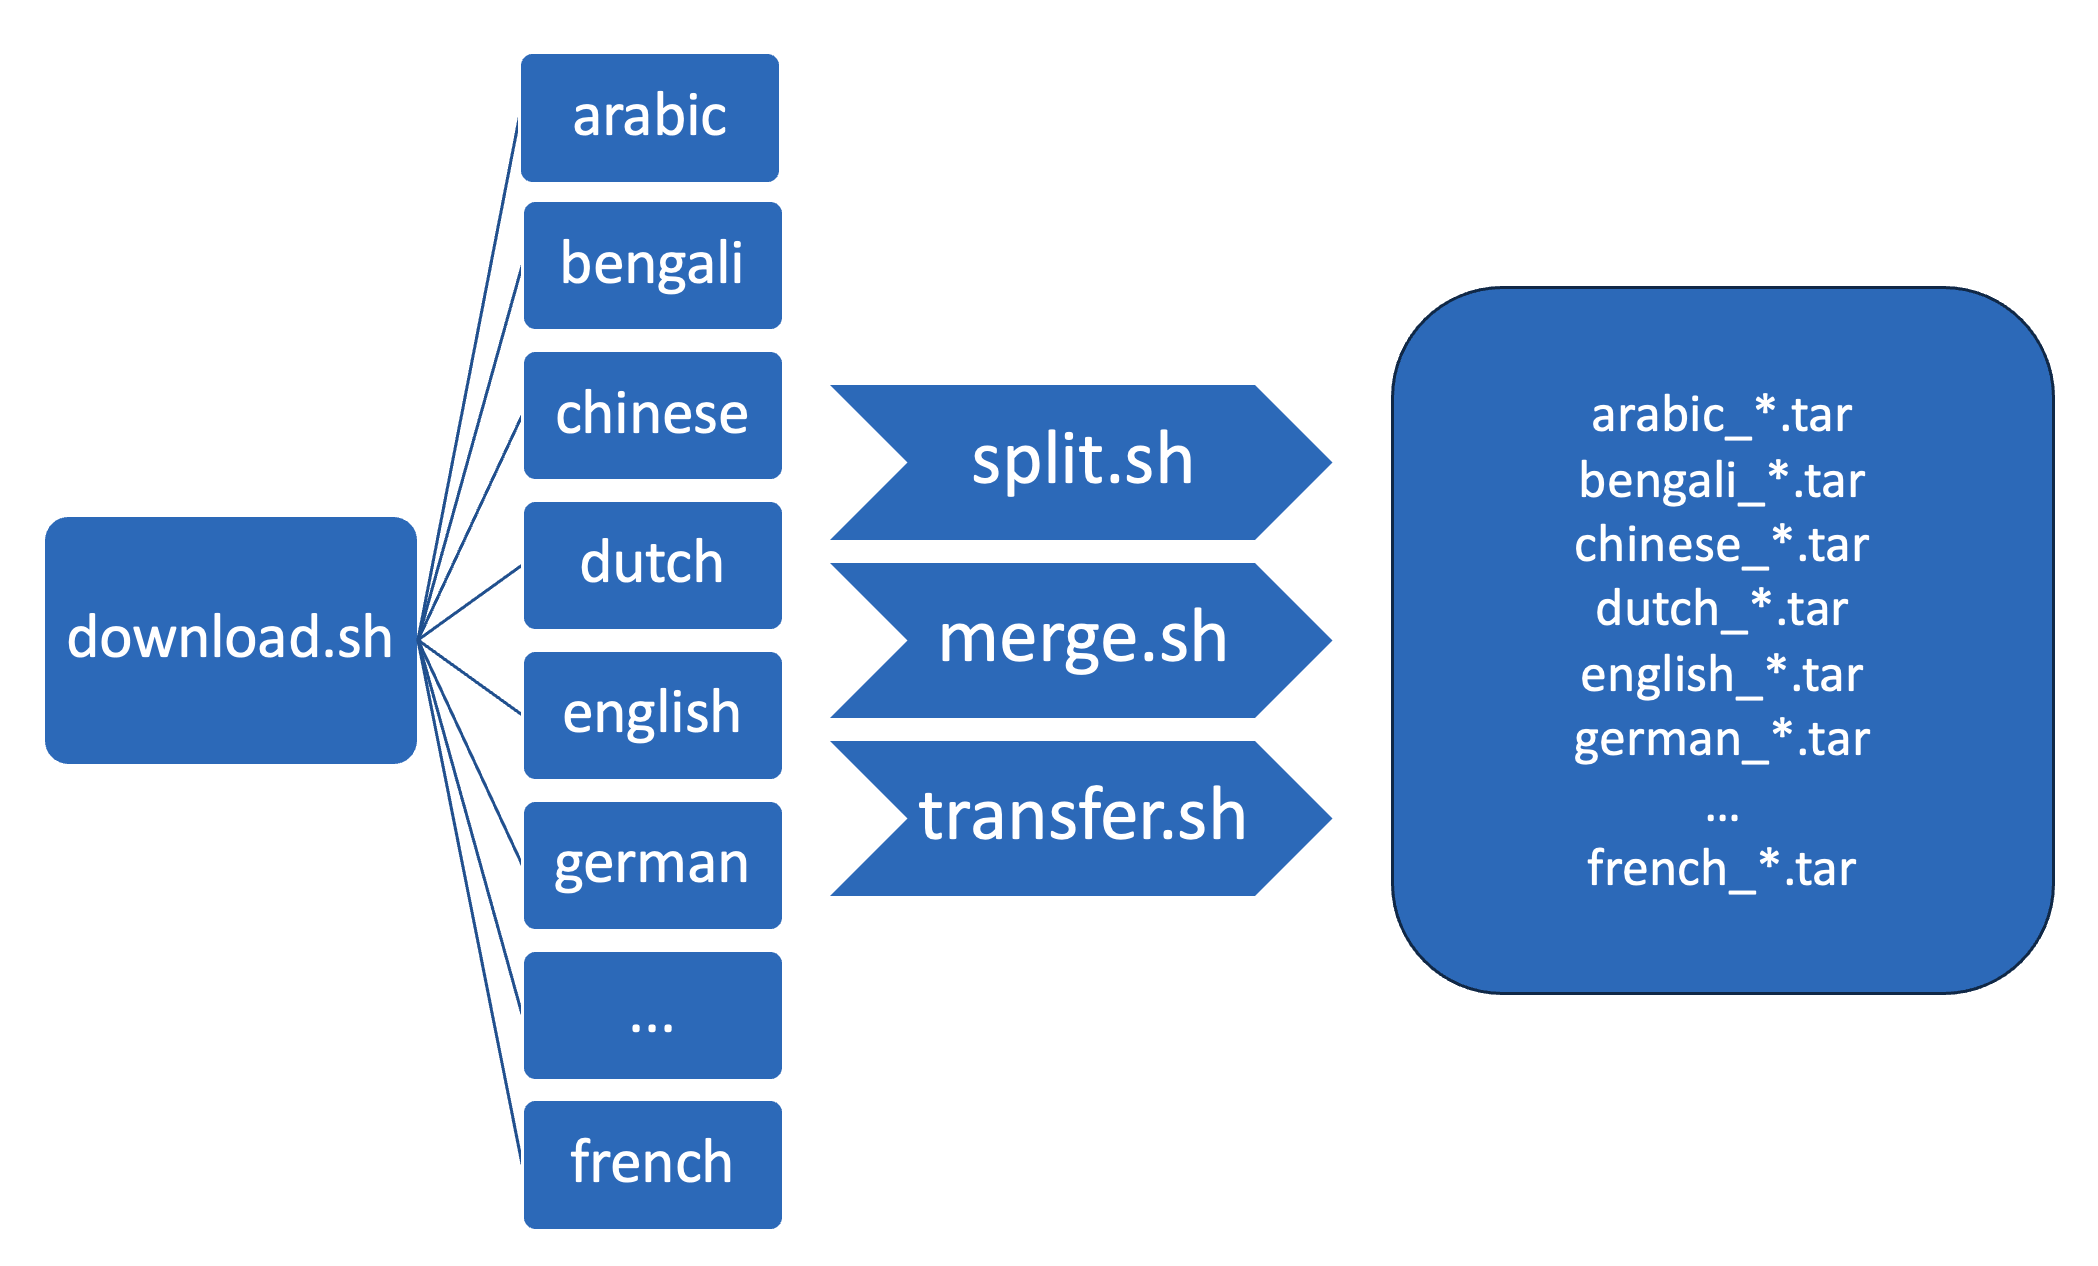
\includegraphics[scale=0.3]{data_engineering.png}
    \caption{Flowchart describing downloading parallel processes used.}
\end{figure} 

\newpage
\section{Data Engineering}

Audio files were loaded, and sound features were extracted using the \texttt{librosa} package in python. The features used throughout the project include root mean squared energy, zero crossing rate, spectral flatness, mel-frequency cepstral coefficients, and chroma short-time fourier transforms. For each of those features, the mean, standard deviation, minimum, maximum, first quartile, third quartile, and skew statistics were chosen. To make the features usable for \texttt{sklearn} and \texttt{tensorflow}, relevant procedures such as standardization, feature stacking, dimension reduction, and dataframe creation were done using \texttt{numpy} and \texttt{pandas}. Furthermore, other packages like \texttt{os}, \texttt{glob}, and \texttt{shutil} were used to conduct OS and command line functionalities.

\begin{figure}[h]
    \centering
    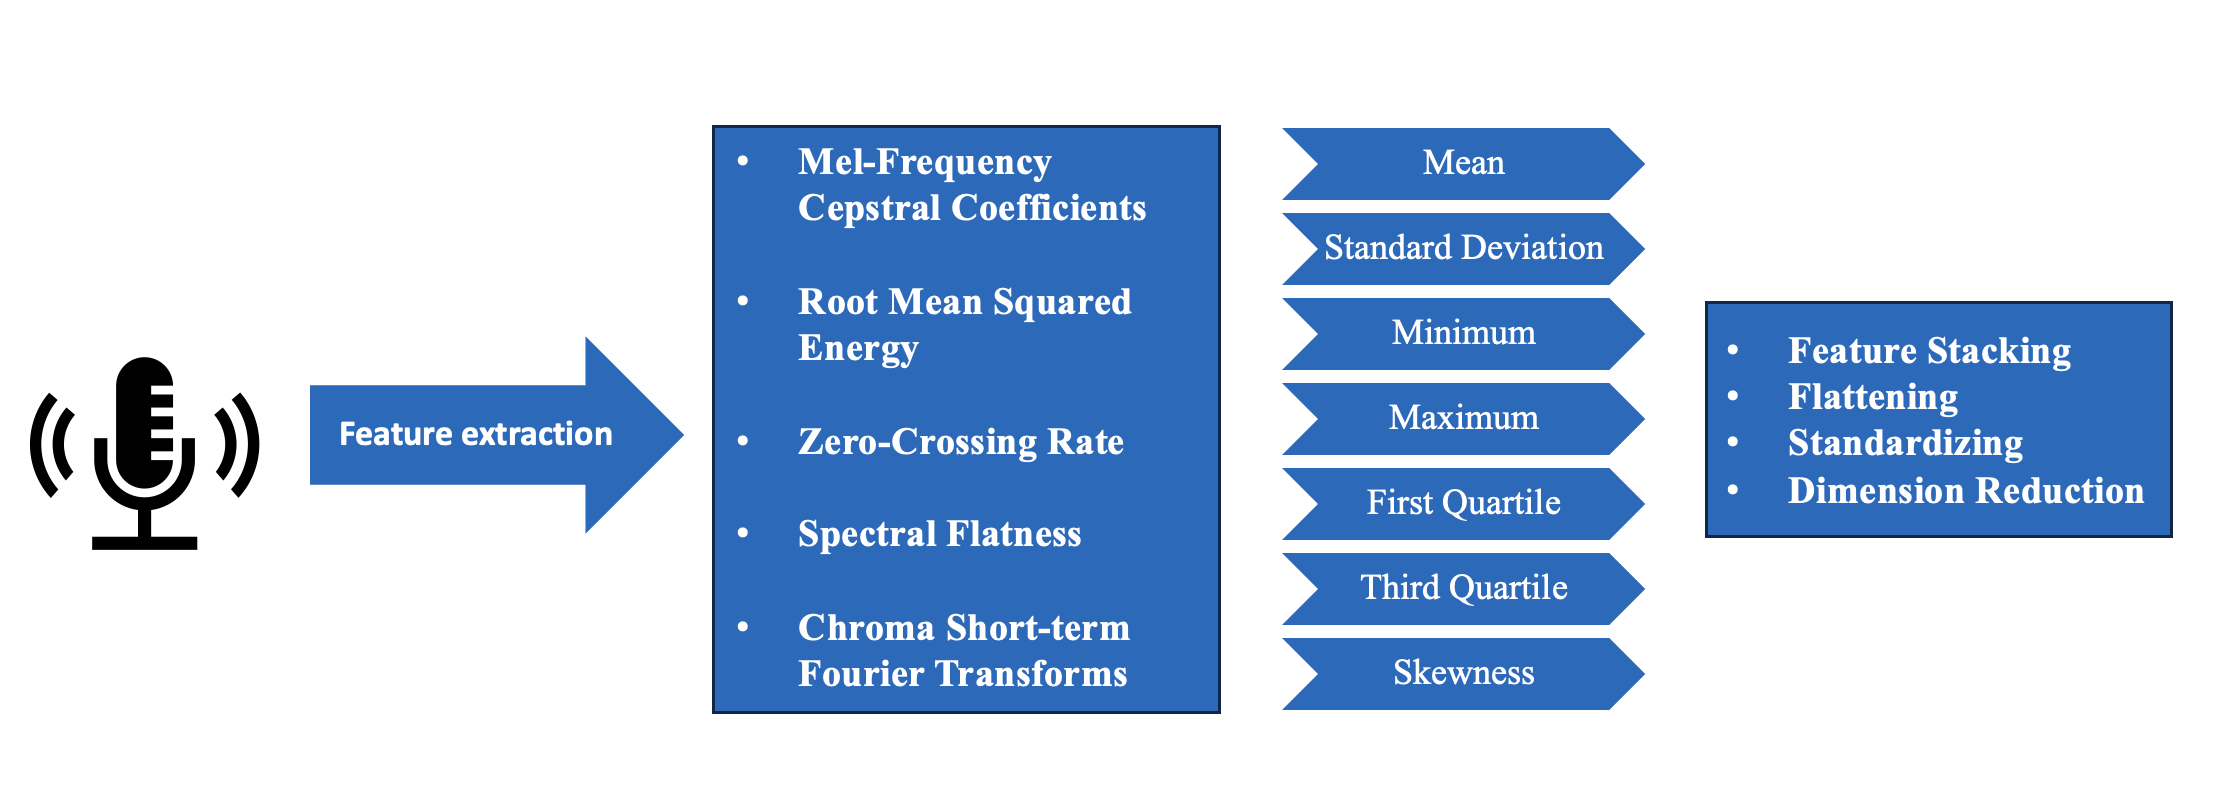
\includegraphics[scale=0.35]{flowchart.png}
    \caption{Flowchart describing engineering procedures used.}
\end{figure} 

\newpage
\section{Outlier Detection to Find Anomalies.}

A combination of two unsupervised outlier detection methods were used for this project. First, Isolation Forests (IF) detected anomalies by utilizing binary trees to recursively generate sub-samples to segment and search for outliers in the data, without employing any distance or density measures. Secondly, a Local Outlier Factor (LOF) was used to compute the local density deviation of a given data point with respect to its neighbors and identify outliers. \texttt{sklearn}'s IF and LOF functions were used for our project, and the intersection of these was used to classify audio as outliers or typical.

\begin{figure}[h]
    \centering
    \includegraphics[scale = 0.355]{newplot(4).png}
    \caption{2D PCA projection with anomalies for a single tar file.}
\end{figure} 

\newpage
\section{Speech Detection}

For the outlier audio found by the ensemble algorithm described above, we ran a preliminary detection procedure to determine whether speech was present in the audio file. To conduct this, a moving average (given parameters: window, stride, and threshold) was taken of the original sound signal waveform, and the following algorithm was run:

\[\xi(\vec{\mu}) = 
\begin{cases}
    \text{False} & \text{if}\;\;|\text{max}_{i} - \text{min}_{i}| < \text{threshold} \\
    \text{True} & \text{Otherwise}
\end{cases}\]

\noindent If $\xi(\vec{\mu}) = \text{False}$, no speech detected (and the audio is removed), otherwise it's de-noised.

\begin{figure}[h]
    \centering
    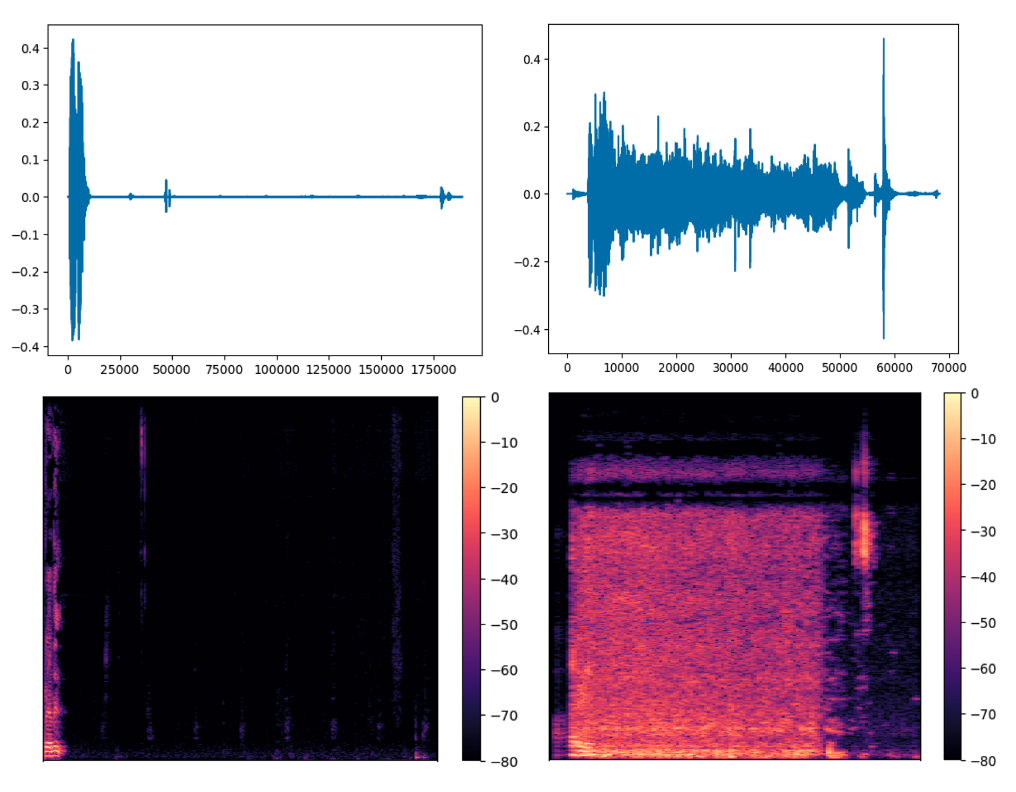
\includegraphics[scale = 0.5]{silent.png}
    \caption{Examples of audio files with no speech.}
\end{figure} 

\newpage
\section{De-noising using spectral gating}

For outlier audio with detected speech, a de-noising algorithm was applied using spectral gating via the \texttt{noisereduce} package, for which our high-level understanding includes the following as a few main steps:

\begin{enumerate}
  \item Calculate Fast-Fourier Transforms (FFT).
  \vspace{-0.5cm}
  \item Calculate Statistics on Result.
  \begin{itemize}
  \vspace{-0.5cm}
     \item  Use resulting "power" vector and its statistics to calculate a threshold for filtering.
  \end{itemize}
  \vspace{-0.5cm}
  \item "Mask" is smoothed and reapplied, inverted, to the FFT of the signal to produce a "cleaned" result.
  \vspace{-0.5cm}
\end{enumerate}
\centerline{\textit}
\begin{figure}[h]
    \centering
    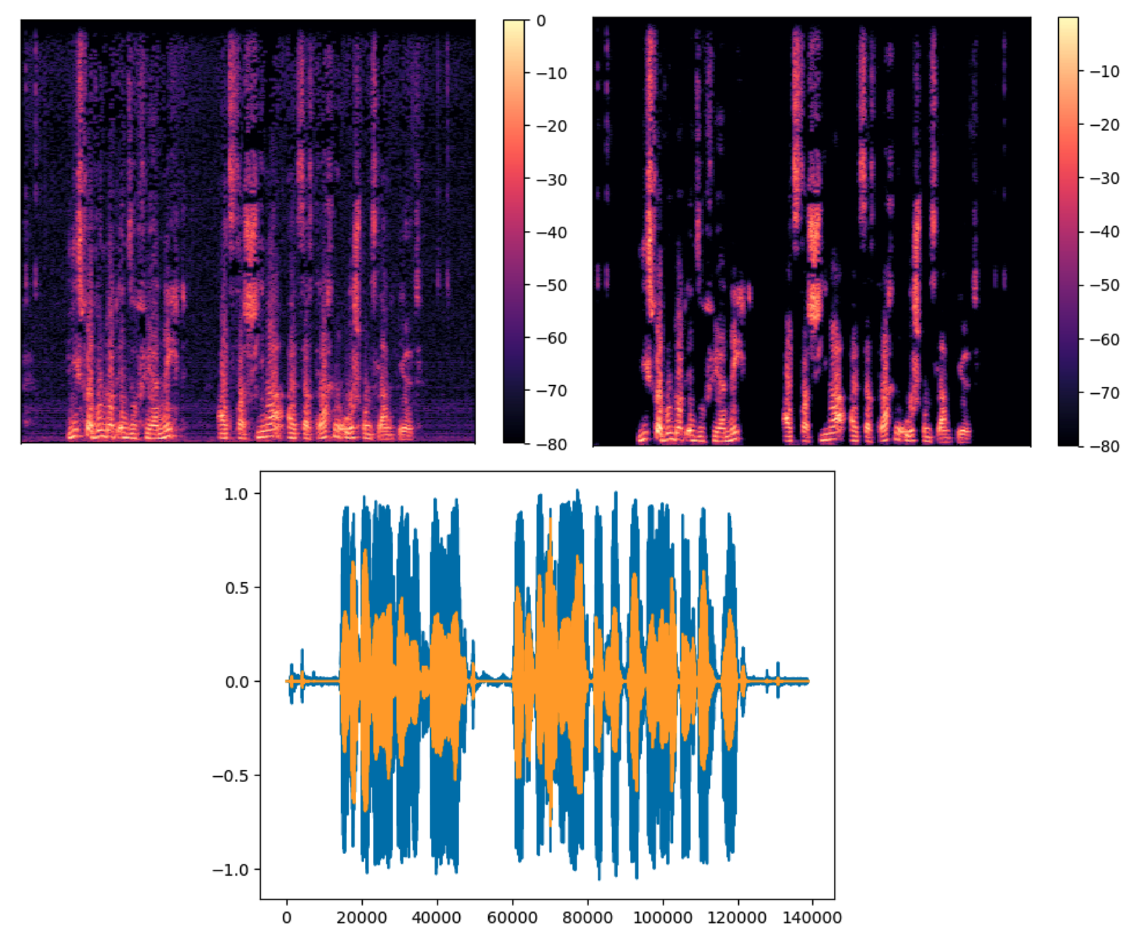
\includegraphics[scale = 0.5]{denoising.png}
    \caption{Examples of audio files that needed de-noising (before and after).}
\end{figure} 

\newpage
\section{Metrics}

To analyze the effectiveness of our speech enhancement process, we created two Convolutional Neural Network (CNN) Models trained on both clean or unclean data and compared their performances.

\begin{figure}[h]
    \centering
    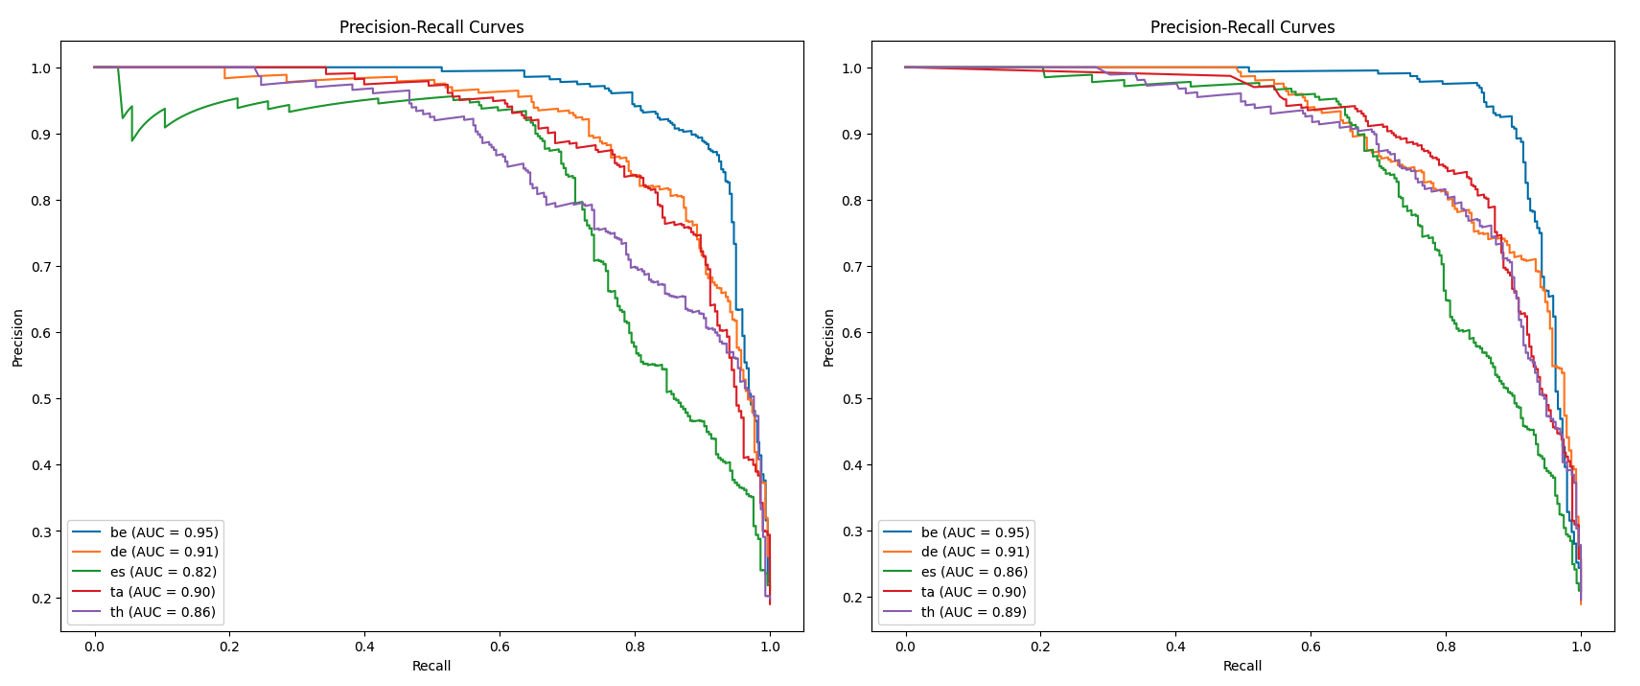
\includegraphics[scale = 0.5]{auc_recall.png}
    \caption{Precision Recall Curves (left: before cleaning, right: after cleaning).}
\end{figure} 

\begin{figure}[h]
    \centering
    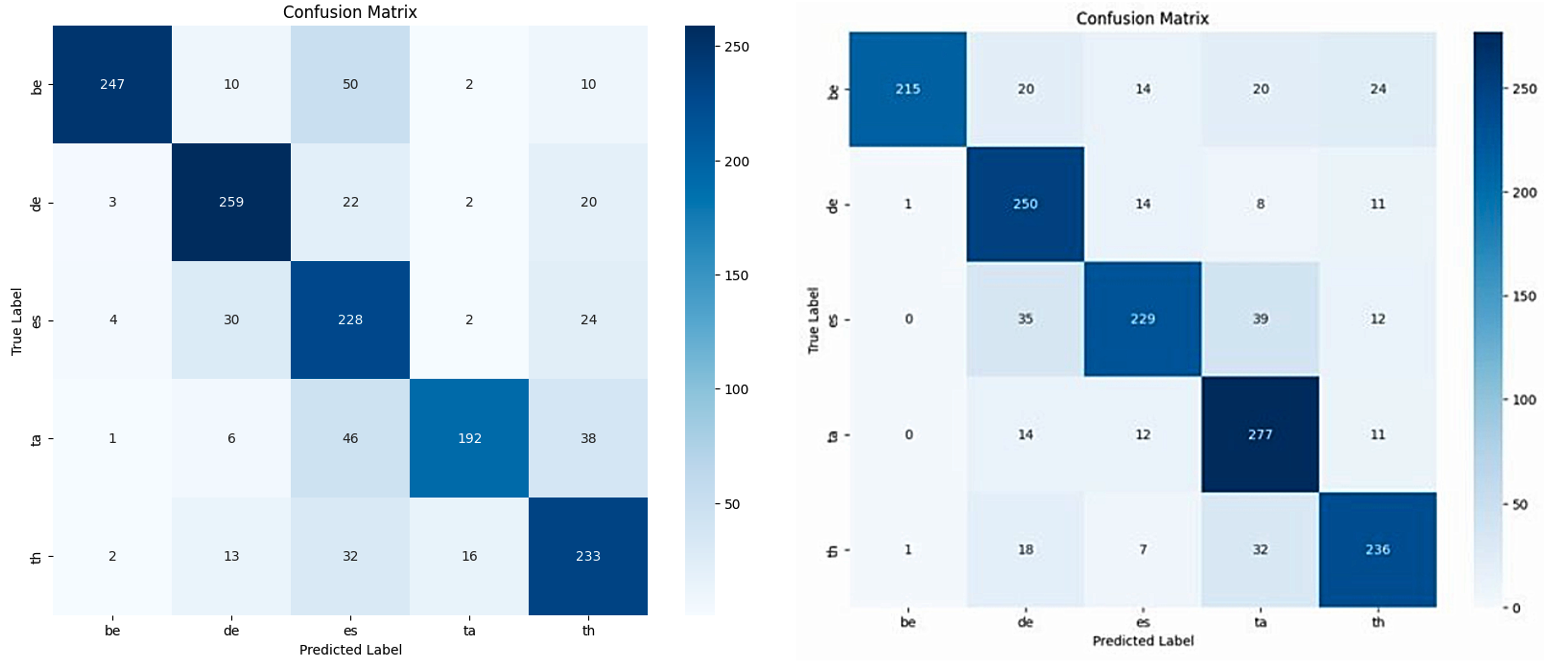
\includegraphics[scale = 0.5]{confusion.png}
    \caption{Confusion matrices (left: before cleaning, right: after cleaning).}
\end{figure} 

\newpage
\section{Conclusion}

\noindent For only 7500 audio files and 5 hand-picked languages - Bengali, German, Spanish, Tamil, and Thai - the overall test accuracy increased by 2\%. Furthermore, the AUC score either remained unchanged or increased across the board (the curves also showed more consistent results and sharper trends) and the confusion matrix displayed a higher accuracy (as can be seen by consistently darker diagonal and consistently lighter non-diagonal elements). Subsequently, we conducted this speech enhancement algorithm for all audio files across every language by running 1320 parallel jobs for each tar file.

\newpage
\section{References and Appendix}

\noindent Breunig, Markus M. and Kriegel, Hans-Peter and Ng, Raymond T. and Sander, J (2000). LOF: Identifying Density-Based Local Outliers. Association for Computing Machinery. New York, NY, USA. \url{https://doi.org/10.1145/335191.335388}.\\

\noindent Ji Wu, Fei Yang, Wenkai Hu (2023). Unsupervised anomalous sound detection for industrial monitoring based on ArcFace classifier and gaussian mixture model. Applied Acoustics. \url{https://doi.org/10.1016/j.apacoust.2022.109188}\\

\noindent Liu, Fei Tony and Ting, Kai Ming and Zhou, Zhi-Hua (2012). Isolation-Based Anomaly Detection. Association for Computing Machinery. New York, NY, USA. \url{https://dl.acm.org/doi/10.1145/2133360.2133363}.\\

\noindent Lo Scudo, F., Ritacco, E., Caroprese, L. et al. Audio-based anomaly detection on edge devices via self-supervision and spectral analysis. J Intell Inf Syst (2023). \url{https://doi.org/10.1007/s10844-023-00792-2}\\

\noindent Sainburg T. timsainb/noisereduce: v1.0.1; 2019. \url{https://github.com/timsainb/noisereduce}. Available from: \url{https://doi.org/10.5281/zenodo.3243589}.\\


\end{document}
